\documentclass{article}
\usepackage{amsmath}
\usepackage{hyperref}
\usepackage{graphicx}
\begin{document}
\tableofcontents
\section{Introduction}
In this report, we implemented some regression models to fit the data within two datasets, including the linear regression, random forest regression, neural network regression and polynomial regression. We made some comparisons between the prediction results of different models based on root mean squared error(RMSE) and the coefficient of determination($R^2$).
Based on the statistics provided by models, we analyzed the significance of different features. In order to avoid overfitting, which often happens in the regression fitting problem, we implemented both cross-validation and regularization techniques. Moreover, since some of the features have no numerical meaning, we formatted them into binary features, which increase the number of features. \\
\\
The report is organized as follows : In section 2, we preprocessed the data and plotted the data to find some pattern. In section 3, The dataset was from a simulated traffic data on the backup system in a networkwe. We implemented both the linear regression model and random forest regression model to predict the copy size of the backup file and made some analysis and comparisons of the predictions. In section 4, we implemented the neural network model and polynomial regression model to fit the data and analyzed the impact of different parameters to the results. In section 5...
\section{Data Preprocessing}
After checking the data, there are seven features in the dataset named network\_ backup\_ dataset, including week, day of the week, backup start time, work flow ID, file name, size of backup and backup time. The target value is the size of backup, others are features. Therefore, first of all we need to transform non-numerical values into numerical values. However, consider "the day of the week" feature, "Tuesday" is not larger than "Monday", but "2" is larger than "1". So we need to make such kind of features into binary format. For instance, for "day of the week", we need to expand it into seven features, where it is 1 on the specified day and all the others 0. Finally, we have 64 features in total.\\
\\
In order the find the pattern, we plot the figure of the copy size over time. The independent variable is the "Start Time - Hour of Day", the dependent variable is the copy size. There are six sampling times in a day and 20 days as a period. So the x axis is from 1 to 120. The figure is shown in figure \ref{fig:start_time}.
\begin{figure}[htbp]
\centering
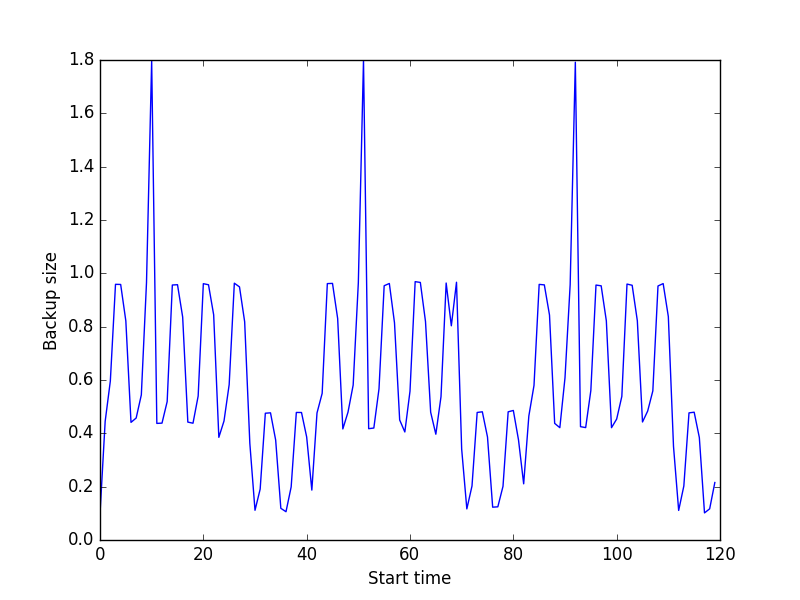
\includegraphics[width=.6\textwidth]{pattern_start.png}
\caption{The copy size of backup over start time}
\label{fig:start_time}
\end{figure}
From \ref{fig:start_time} we can see there is clearly a cycle between copy size and time. So we plot the copy size over days to find the cycle period. The result is shown in figure \ref{fig:day}. Hence we can predict that the cycle period is approximately a week.
\begin{figure}[htbp]
\centering
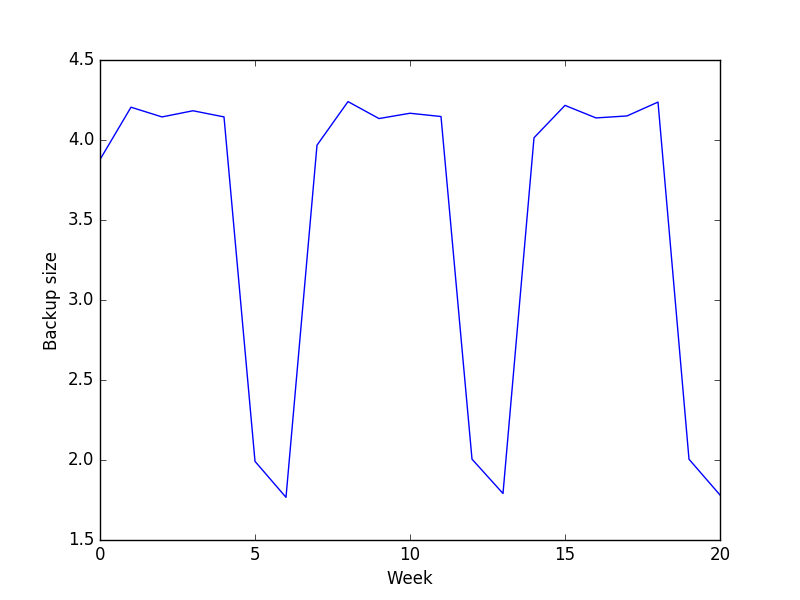
\includegraphics[width=.6\textwidth]{pattern_week.png}
\caption{The copy size of backup over week}
\label{fig:day}
\end{figure}
\section{Linear and Random Forest Regression}
In the Linear Regression Model, we choose the copy size as the target variable and the other attributes as the features, the fit model is as follow
\begin{equation*}
\bar{Y} = X\alpha
\end{equation*}
where $\bar{Y}$ represents the target, $X$ represents the features vector and $\alpha$ is the linear coefficient. We used least square as the penalty function, which is
\begin{equation*}
min || Y - \bar{Y} ||_2
\end{equation*}
In order to avoid the overfitting problem, we implemented 10-fold cross-validation technique. First do a random shuffling over the data, then split them into 10 folds. Each time choose 9 of 10 as the train set and the other 1 fold as the test set. The Root Square Mean Error (RMSE) is shown in figure \ref{fig:rmse_lr}. The average RMSE is 0.071.
\begin{figure}[htbp]
\centering
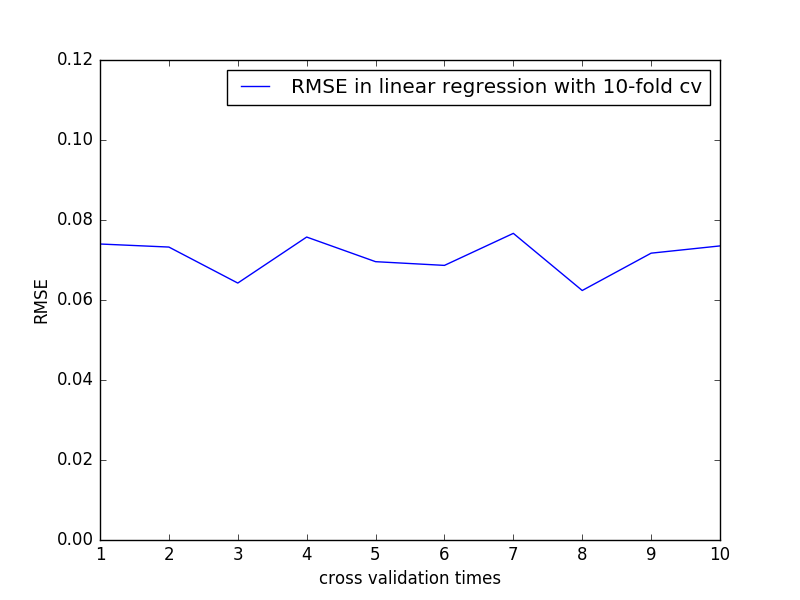
\includegraphics[width=.6\textwidth]{rmse_linear.png}
\caption{The copy size of backup over week}
\label{fig:rmse_lr}
\end{figure}
To evaluate the fitting accuracy of our model, “Fitted values VS actual values” and “residuals vs fitted values” are plotted. From figure \ref{fig:actual_pred}, we can see that most predicted values are close to the actual values. From figure \ref{fig:residual}, we can see that the residuals are distributed randomly around zero axis, which means the model is proper.\\
\begin{figure}[htbp]
\centering
\begin{minipage}[t]{0.45\textwidth}
\centering
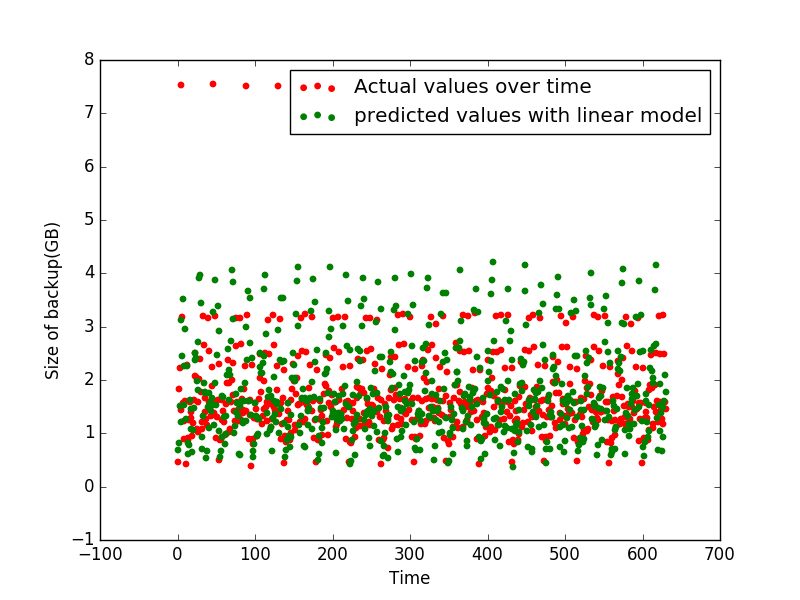
\includegraphics[width=\textwidth]{actual_pred.png}
\caption{Actual VS predicted}
\label{fig:actual_pred}
\end{minipage}
\begin{minipage}[t]{0.45\textwidth}
\centering
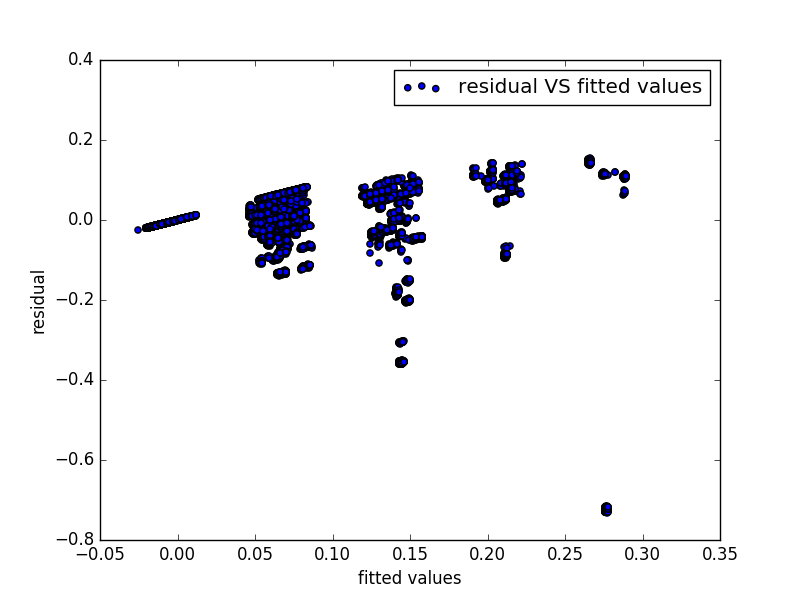
\includegraphics[width=\textwidth]{residual.png}
\caption{Residual VS fitted values}
\end{minipage}
\label{fig:residual}
\end{figure}
\\
As for the significance of different variables, we choose p-value as the evaluation criterion. The p-value of the six features is shown in figure \ref{fig:p6}.\\
\begin{figure}[htbp]
\centering
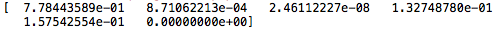
\includegraphics[width=.8\textwidth]{pvalue-6.png}
\caption{p-value of 6 features}
\label{fig:p6}
\end{figure}
\\
Therefore the most important two features are "Backup start time - Hour of the day" and "Backup Time" because their p-values are close to 0.
For 64 features, the p-value matrix is shown below.\\
\begin{figure}[htbp]
\centering
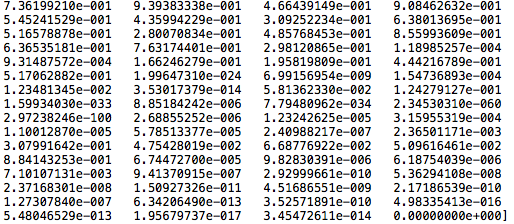
\includegraphics[width=.8\textwidth]{pvalue-64.png}
\caption{p-value of 64 features}
\label{fig:p64}
\end{figure}
\\
For random forest regression, we initialize the model with parameters : number of trees 20, depth of trees 4. The average RMSE is 0.0297. After tuning the parameters, we have the best RMSE 0.00943. The best RMSE is shown in figure \ref{fig:rf}.\\
\begin{figure}[htbp]
\centering
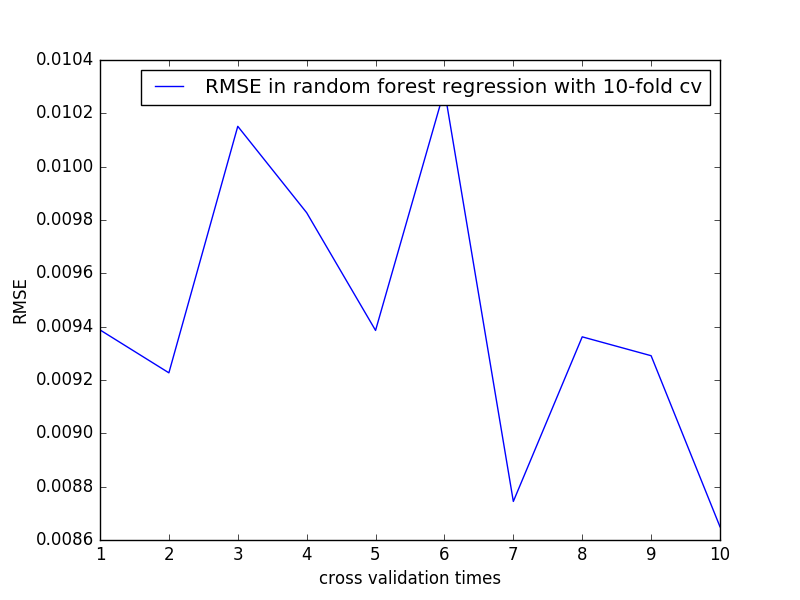
\includegraphics[width=.6\textwidth]{rf_rmse.png}
\caption{The best RMSE of random forest regression}
\label{fig:rf}
\end{figure}
\\
The comparison between Linear Regression and Random Forest Regression is shown in figure \ref{fig:comp}. Random forest is a lot better than linear regression.\\
\begin{figure}[htbp]
\centering
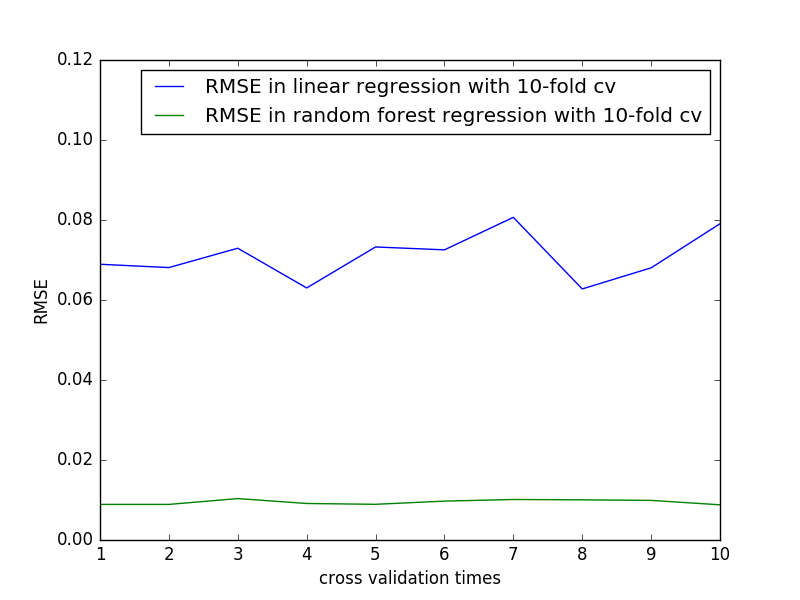
\includegraphics[width=.6\textwidth]{compare.png}
\caption{The comparison between Linear and Random Forest Regression}
\label{fig:comp}
\end{figure}
\\
The prediction of the random forest model is shown in figure \ref{fig:r_pred}. We can see the cycle period is around 42 backup times, which is about a week, so the pattern is the same with the actual values.
\begin{figure}[htbp]
\centering
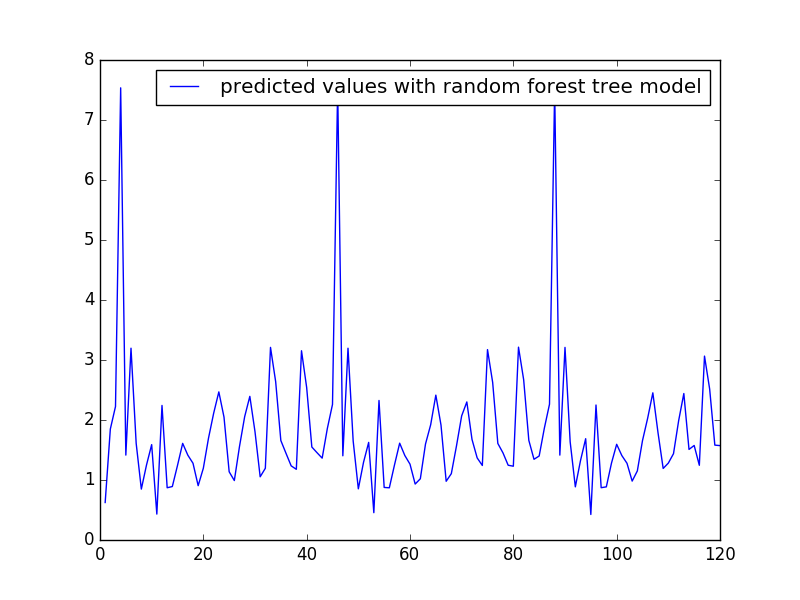
\includegraphics[width=.6\textwidth]{random_pred.png}
\caption{The prediction of the random forest}
\label{fig:r_pred}
\end{figure}
\section{Neural Network}
In the neural network model, we choose the feedforward network with the backpropagation trainer. The main parameters are the number of layers, the kind of hidden layers and the number of iteration before convergence. After lots of experience, we find that sigmoid layer is proper for hidden layers and linear layer is proper for the output layer. The optimal number of layers is 7. The RMSE reduces when the number of iteration is increasing, however it is too slow with large iteration number. So we set it to be 10. The best RMSE we can get is 0.827. The RMSE is shown in figure \ref{fig:nn}.
\begin{figure}[htbp]
\centering
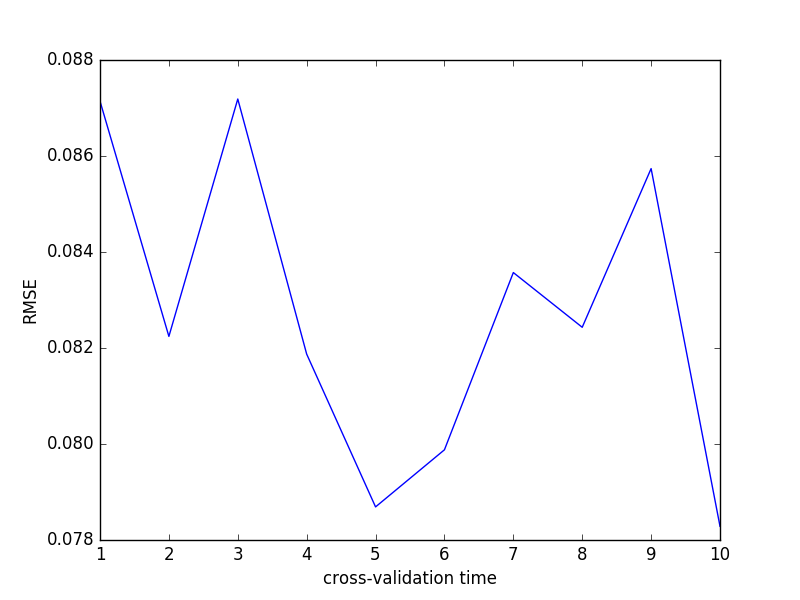
\includegraphics[width=.6\textwidth]{nn.png}
\caption{The RMSE of neural network model}
\label{fig:nn}
\end{figure}
\end{document}